\documentclass[man, 12pt]{apa7} % 'man' for manuscript, 12pt font size


\usepackage[american]{babel} % American English
\usepackage{csquotes} % Recommended with biblatex
\usepackage{pdflscape}


% Bibliography setup for APA style
\usepackage[style=apa, sortcites=true, sorting=nyt, backend=biber]{biblatex}
\addbibresource{mahbod.bib} % Your .bib file
\DeclareLanguageMapping{american}{american-apa}

% Additional useful packages
\usepackage{graphicx} % For including graphics
\usepackage{booktabs} % For professional quality tables
\usepackage{amsmath} % Enhanced math support
\usepackage{amsfonts} % Additional math fonts
\usepackage{amssymb} % Extended symbol collection
\usepackage{hyperref} % For hyperlinks in the document
\usepackage{pcl}
\usepackage{booktabs}
% Margins and spacing adjustments if needed
\usepackage{geometry}
\geometry{
    left=1in,
    right=1in,
    top=1in,
    bottom=1in
}
\usepackage{setspace}
\doublespacing % or \onehalfspacing

% Title, authors, and affiliations
\title{Estimating Correlations in Low-Reliability Settings With Constrained Hierarchical Models}
\shorttitle{Constrained Hierarchical Models}
\author{Mahbod Mehrvarz, Jeffrey N. Rouder}
\affiliation{{University of California, Irvine}}


% Author note
\authornote{
    Version 1, February, 2024.
    
    \addORCIDlink{MM}{0009-0002-5426-5867}
    
    \addORCIDlink{JNR}{0000-0003-2023-3891} 
    
    Author Contributions: MM and JNR jointly conceived the project, developed the models, executed the simulations, and wrote the results.

    Open Science Practices: The simulated data, analysis scripts, and code used to generate the figures are openly available at \href{https://github.com/specl/ctx-pca-localize}{https://github.com/specl/ctx-pca-localize}
    
    This research was supported in part by NSF 2126976 and by ONR N00014-23-1-2792.

    Correspondence concerning this article should be addressed to Mahbod Mehrvarz, Department of Cognitive Sciences, University of California, Irvine, CA, 92697. E-mail: mehrvarm@uci.edu
}



% Abstract and Keywords
\abstract{
It is popular to study individual differences in cognition with experimental tasks, and the main goal of such approaches is to analyze the pattern of correlations across a battery of tasks and measures.  One difficulty is that experimental tasks are often low in reliability as effects are small relative to trial-by-trial variability.  Consequently, it remains difficult to accurately estimate correlations.  One approach that seems attractive is hierarchical modeling where trial-by-trial variability and variability across conditions, tasks, and individuals are modeled separately.  Here we show that hierarchical models may reduce the error in estimating correlations up to 46\%, but only if substantive constraint is imposed.  The approach here is Bayesian, and we develop novel Bayesian hierarchical factor models for experiments where trials are nested in conditions, tasks, and individuals.  The prior on covariances across tasks can either be unconstrained, in which there is little error reduction, or constrained, in which there is substantial error reduction.  The constraints are: 1. There is a low-dimension factor structure underlying the covariation across tasks; and 2. All loadings are nonnegative leading to a positive manifold on correlations.  We argue that both of these assumptions are reasonable in cognitive domains, and that with them, researchers may profitably use hierarchical models to estimate correlations across tasks in low-reliability settings.
}

\keywords{Individual Differences, Cognitive Control, Methodology, Factor models, Bayesian Hierarchical Models}


\begin{document}

\maketitle

In the modern landscape, researchers study cognitive abilities such as perception, language, problem-solving, and memory through the lens of information processing. The main focus is on understanding how we represent, manage, combine, store, recall, and assess information from our surroundings.  These abilities are often measured in experiments comprised of conditions that are contrasted to eliminate nuisance factors. For example, to measure \textbf{cognitive control}--the ability to inhibit proponent responses--tasks such as Stroop employ congruent and incongruent conditions. The difference in response times between the two conditions serves as a measure of cognitive control without the influence of factors that generically affect response times.  In this manner, the experimental approach with contrasted conditions provides for theoretically valid and interpretable measures of cognitive abilities. 

Over the last century, researchers have used individual differences across tasks to understand underlying mental processes and variations in them across populations.  Continuing with the cognitive control example, we note that the structure and correlates of cognitive control have been studied repeatedly with individual differences using experimental tasks. However, finding consistent patterns of individual differences has proven difficult. 

This difficulty perhaps reflects a statistical concern that goes by the moniker of the \textbf{reliability crisis}. Indeed, measures of cognitive abilities from experimental designs often lack sufficient reliability for latent variable modeling. Three characteristics observed in recent inquiries have exemplified this concern: First, several tasks that purportedly measure the same construct do not correlate well. For example, the correlation between flanker and Stroop effects in large studies is often near .1 and rarely greater than .25. \parencite{Enkavi.etal.2019, Rey-Mermet.etal.2019, Rouder.etal.2023}. Second, factor-model analyses have not proven replicable or robust.  The evidence comes from \Textcite{Karr.etal.2018}, who showed that when bootstrapped simulated data were submitted to confirmatory-factor-model analysis, the best-fitting model from the original set was rarely recovered. Finally, it has been observed that individual differences in experiments have low reliability \parencite{Hedge.etal.2018, Draheim.etal.2019}.  How people differ in an experiment does not predict with high precision how they will differ again.

How bad is this reliability problem?  The following brief example may serve as motivation.  Consider an experiment with six tasks.  Each task is comprised of two conditions---a congruent and an incongruent condition---with the latter requiring more cognitive control than the former.  In this setup, trials are nested in conditions; for instance, an individual might perform 100 trials in each condition for each task. The focal point of interest here is the individual's score, calculated as the difference in average performance between the incongruent and congruent conditions, and the critical question is how these scores covary across the tasks. With six tasks at hand, we encounter 15 distinct inter-task correlations. For simplicity, let's posit that each task correlates with every other task at a true value of $\rho=.5$. This value is depicted in the first column of Figure \ref{fig:prob_setup}A, labeled \textit{Truth}. We simulated data from this setup for 200 hypothetical individuals using realistic values for true performance (details to be discussed later). The next column, labeled \textit{Usual}, is the usual Pearson sample correlation estimate from individuals' scores.  Note that these sample correlations are dramatically underestimated.  Indeed, this attenuation of correlation is a well-known phenomenon that occurs when scores are particularly prone to measurement error \parencite{Spearman.1904}.  A challenging aspect of this attenuation is that it is \textbf{asymptotic}.  As the number of individuals in the experiment is increased, attenuation does not decrease.  Rather, the analyst becomes increasingly confident in badly attenuated values.


One long-standing strategy to mitigate attenuation is to calculate how much attenuation may be present and adjust accordingly; this process is called \textbf{disattenuation}.  The third column in Figure \ref{fig:prob_setup}A shows Spearman's correction\footnote{Spearman's correction for attenuation is $r^*_{xy} = \frac{r_{xy}}{\sqrt{r_{xx}\cdot r_{yy}}}$ where $r_{xy}$ is the Pearson sample correlation between two variables, and $r_{xx}$ and $r_{yy}$ is the reliability of each.} for attenuation \parencite{Spearman.1904} for the 15 intertask correlations. As advertised, these corrected values are disattenuated and center around the true value.  Yet, these values are surprisingly variable.  The experiment simulated here is quite large comprising 240,000 observations from 200 individuals performing 100 trials across two conditions in six tasks.  One might expect that estimates of 15 correlation coefficients from 240,000 observations would be highly accurate. However, the reality is strikingly different: the disattenuated correlations range widely from .2 to .8, deviating on average by .18. The extent of uncertainty in such a large data set is disconcerting. This inability to localize correlations in reasonable cognitive-control settings serves as the problem for this report.

Why is localizing these correlations important?  There are two reasons.  First, the correlation (or covariation) among tasks serves as a critical target for capturing the relations among tasks.  Second, this covariation is often decomposed using latent variable models such as factor analysis and structural equation modeling.  The effectiveness of these latent variable decompositions hinges critically on the precision with which these correlations may be localized. In cases where correlations are imprecisely localized or dramatically attenuated, the resulting latent structure may be only weakly identifiable, casting doubt on the validity of inferences drawn from it \parencite{Karr.etal.2018}.

Several recent approaches have been proposed to address the issue of poor localization.  \textcite{Draheim.etal.2019} recommends measures that do not depend on contrasting conditions. \textcite[]{Deveau.etal.2015, Kucina.etal.2023, Wells.etal.2021} recommend gamification where experiments are integrated into an engaging computer video game format complete with stimulating music and a competitive points system.  \textcite[]{Haines.etal.2023,Matzke.etal.2017,Rouder.Haaf.2019} recommend hierarchical model analysis where multiple sources are modeled separately.  Hierarchical modeling approaches are explored here.

Yet, from our experience, the anticipated benefits of hierarchical models in localizing correlations have not fully materialized. \textcite{Rouder.etal.2023} used a simulation approach to assess whether hierarchical models could indeed localize correlations in reasonable designs with realistic effects. The fourth column of Figure \ref{fig:prob_setup}A, labeled {\em Unconstrained} shows correlations from a hierarchical model, to be presented subsequently. Rouder et al. identified three key advantages of the hierarchical approach.  First, hierarchical-model analysis typically leads to less attenuation compared to the usual approach. Second, it achieves somewhat more precise localization than Spearman's disattenuation method in repeated simulations \parencite[]{Rouder.etal.2023}. Third, hierarchical models offer a realistic assessment of uncertainty in correlations. The last benefit is illustrated in Figure \ref{fig:prob_setup}B. The histogram is the posterior distribution of one of the correlations. The dashed lines show the $95\%$ credible interval.  This interval is large, spanning from .27 to .76 in value.  Its size shows the high degree of uncertainty, which reflects a high degree of variability in performance from trial to trial.  In contrast, the usual estimate is shown as a point.  The segments show the  $95\%$ confidence interval.  The relatively narrow confidence interval reflects the large number of individuals without consideration of trial-to-trial variability. The usual correlation is greatly attenuated (true value is .5) indicating that this high level of confidence is misplaced. 

Despite these three benefits, the problem of precise localization of correlations remains.  In experiments of reasonable size, Root Mean Square Error (\textbf{RMSE}) remains high, often around .15, suggesting that even with a large data set of 240,000 observations, discerning whether a correlation was .3 or .7 remains elusive.  Localizing correlations even with hierarchical models is challenging even in large data sets.


\section{Constrained and Unconstrained Hierarchical Models}

One strategy for increasing the precision of estimates is to use simpler and more constrained models.  An example of this strategy comes from polynomial regression: the slope of a regression term will be estimated to higher precision when higher-order terms are excluded from the model.  We propose using constrained hierarchical models that are designed to increase the precision of estimating covariation.  The approach, of course, is not cost free---the constraints we impose have to be realistic and warranted.  The constraints we explore are a positive manifold across covariation and a low-dimensional factor structure across tasks.

This pay-to-play strategy is best explained with the formal specification of models.  Consider a battery of cognitive control tasks where $I$ individuals each perform $J$ tasks. Each task is comprised of a congruent and an incongruent condition, and each individual performs $L_{ijk}$ trials in each condition. Let $i=1,\ldots,I$ index individuals, $j=1,\ldots,J$ index tasks, $k=1,2$ index conditions, and $\ell=1,\ldots,L_{ijk}$ index replicate trials. Let $Y_{ijk\ell}$ denote an observation, for example, the response time on a given trial.  We place the following linear model on $Y$:
\begin{equation} \label{eq:RT_surface}
Y_{ijk\ell} = \alpha_{ij} + x_k\theta_{ij} + \epsilon_{ijk\ell}.
\end{equation}

In this model, $x_k$ is the contrast code for the two conditions, set at -$\frac{1}{2}$ and $\frac{1}{2}$ for congruent and incongruent conditions, respectively. The parameter $\alpha_{ij}$ is the true overall speed of the $i$th individual on the $j$th task. The parameter $\theta_{ij}$ is the true difference between incongruent and congruent conditions for the $j$th task---it is the $i$th individual's true effect on the $j$th task and is the focal point of analysis.  The error term is $\epsilon_{ijk\ell} \sim \mbox{Normal}(0,\tau_j^2)$, with $\tau_j^2$ describing the variability of trial noise for the $j$th task. Errors are independent of one another. 

At the next level, we place random effect models on individual true effects.  Let $\bftheta=(\theta_{i1},\ldots,\theta_{iJ})'$ be a column vector true effects for the $i$th individual, which is modeled as a multivariate normal:
\begin{equation} \label{eq:true_effect_mat}
\bf{\theta}_i \sim \mbox{N}_J(\bfmu,\bfSigma),
\end{equation}
where $\bfmu=(\mu_1,\ldots,\mu_J)'$ is a vector of mean effects and $\bfSigma$ is a $J \times J$ covariance matrix.  

The target for constraint in this context is the covariance matrix, $\bfSigma$ \parencite[]{Bollen.1989}. In the most general formulation, no constraint is placed on $\bfSigma$ other than it is valid covariance matrix.  When no constraint is placed on $\bfSigma$, then any relations among the tasks may be accounted for.  Constraint may be added by placing restrictions on the elements of $\bfSigma$.  Consider, for example, the constraint from a one-factor model (see Figure ~\ref{fig:fac_st}A).  Under this constraint, the covariance $\bfSigma$ is,
\begin{equation} \label{eq:oneFacVar}
\bfSigma=
\begin{bmatrix}
\sigma^2_1+\lambda_1^2 & \lambda_1\lambda_2 & \lambda_1\lambda_3 &\ldots &\lambda_1\lambda_J\\
\lambda_1 \lambda_2 & \sigma^2_2+\lambda^2_2 & \lambda_1\lambda_3 &\ldots &\lambda_1\lambda_J\\
\vdots & \vdots & \vdots & \ddots & \vdots\\
\lambda_1\lambda_J & \lambda_2 \lambda_J & \lambda_3\lambda_J & \ldots & \sigma^2_J+\lambda^2_J
\end{bmatrix},
\end{equation}
where $\lambda_j$ and $\sigma^2_j$ are the factor loading and residual variance in true effects, respectively, for the $j$th task.  This covariance matrix is highly constrained.  For example, we can express $\mbox{Cov}(3,4)=\mbox{Cov}(1,3)\times\mbox{Cov}(2,4)/\mbox{Cov}(1,2)$ as $\lambda_3\lambda_4=\lambda_1\lambda_3\times\lambda_2\lambda_4/\lambda_1\lambda_2$.   The one-factor constraint entails a reduction in the number of  parameters.  For example, if there are 6 tasks, then the unconstrained covariance matrix has  21 free parameters (6 diagonal elements and 15 off-diagonal elements) while the one-factor constrained version has 12 free parameters.  The critical question then is whether adding constraint on $\bfSigma$ in hierarchical models can substantially improve the localization of correlations in realistic designs.  To foreshadow, we show here that it can.

\section{Hierarchical Models For Estimating Covariation}

The hierarchical models in this report are the combination of Eq \ref{eq:RT_surface} and Eq \ref{eq:true_effect_mat} along with constraints on $\bfSigma$.  These models are analyzed in the Bayesian framework because of computational tractability.  In the Bayesian framework, priors are placed on all parameters.  Our approach here is to use weakly informed subjective priors.  For example, the prior on overall true speed, $\alpha_{ij}$ is a normal with a mean of .8 s and a standard deviation of 1 s.  This specification is quite reasonable for cognitive control tasks like the Stroop or flanker where RTs are typically under a second. Likewise, priors of $\tau$ are broad with much mass between .01 and 1 s, which corresponds to broad prior on standard deviation of trial-to-trial noise with much mass between 100 ms and 1 s.  Likewise, priors on $\mu$ in Eq \ref{eq:true_effect_mat} reflect the expected range of effects between 0 and 150 ms.  The critical specifications are for $\bfSigma$, which follow:


\subsection{The Inverse-Wishart, An Unconstrained Model}

The unconstrained model we use comes from \textcite{Rouder.etal.2023, Haaf.Rouder.2017}.  Here, an inverse Wishart prior is placed on $\bfSigma$: $\bfSigma^{-1} \sim \mbox{Wishart}(m,\bfS)$, where $m$ and $\bfS$ serve as prior settings on the shape and scale of the inverse Wishart.  The shape parameter is uninformative in this context when set to $m=J+1$.  The scale parameter is a bit trickier.  A lack of \textit{a prior} preference for negative or positive correlations comes when $\bfS=b^2\times\bfI$ where $\bfI$ is the identity matrix (of size $J$) and $m\times b^2$ is the expected variance.\footnote{There is an alternative choice of prior for covariance that we extensively explored, the LKJ prior \parencite{Lewandowski.etal.2009}. This prior is less informative than the Wishart because, unlike the Wishart, the estimation of correlation is independent of the specification of scale. Consequently, this prior is recommended \parencite[]{McElreath.2016}, and implementation is convenient in the R-package rstan \parencite[]{Stan_Development_Team2020-sz}. Yet, we found better performance for the inverse Wishart in simulations in that the posterior credible intervals were smaller and better covered the true value. The increased performance of the Wishart reflects the fact that researchers have a rough idea about the scale of individual differences—it is on the order of tens of milliseconds—and this is enough information for the improved performance of the inverse Wishart.}  This expectation is made with reference to the analysis of existing data sets as discussed subsequently.

\subsection{Orthogonal Factor Models}

The orthogonal factor model serves as constraint on $\bfSigma$.  A model of dimension $D$ is given by 
\begin{equation} \label{eq:theta_marg}
\bfSigma=\bflambda\bflambda'+\bfDelta,
\end{equation}
where $\bflambda$ is a $J\times D$ matrix of factor loadings and $\bfDelta$ is a $J \times J$ diagonal matrix with a diagonal of $\sigma_1^2,\ldots,\sigma_j^2$.  If $D=1$, the model reduces to the one-factor model discussed above.  The degree of constraint then is determined by $D$.  When $D=J$, there is no constraint---any covariance may be represented with an equal number of factors to tasks.  As $D$ is reduced, more constraint is added, with the most constraint for $D=1$.  We develop one- and two-factor models here.

The priors for Eq~\ref{eq:theta_marg} are defined as follows. The factor loadings are distributed as $\lambda\sim \mbox{N}(0,.03^2)$, representing a wide-ranging prior. Residual variances $\sigma_j^{2}$ are distributed as $\mbox{Inverse-Gamma}\left(\frac{1}{2},\frac{1}{2}A^2\right)$, where $A^2$ is a prior setting that reflects the scale of variance.  Inverse-gamma distributions with a shape of 1/2 are diffuse and only weakly informative. Additionally, the covariance element ($\bfSigma$) from the Wishart model was tuned in a similar manner.


\subsection{Positive Manifold Constraints}

The positive manifold refers to a well-known finding that cognitive-performance tasks tend to correlate positively.  \textcite{Carroll.1993}, for example, showed that across a large survey of cognitive-performance tasks, people who performed well on one task performed well on the others.  \textcite[p. 25]{Ritchie.2015} dramatically emphasizes the point: "Some researchers have even deliberately creative cognitive tests tapping different skills that they expected not to correlate together, but they always did."  

To implement the positive-manifold constraint, we require that the factor loadings be nonnegative.  This approach is analogous to nonnegative matrix factorization \parencite[]{Lee.Seung.1999}.  In practice, we set a truncated prior $\lambda_{jd}\sim\N_+(0,.03^2)$ 

\subsection{Analysis}

The above hierarchical models were implemented in JAGS \parencite[]{Plummer.2003}.  Many researchers who analyze factor models in the Bayesian framework use the conditional forms of factor models given by $\theta_{ij} \sim \mbox{N}(\mu_j+\sum_d\lambda_{jd}\eta_{id},\delta_j^2)$ \parencite[e.g.][]{Ghosh.Dunson.2009}.  The advantage of using this conditional form is that sampling in MCMC is done through repeated calls of independent normals.  The disadvantage in this context is poor mixing; samples in chains are highly correlated from iteration to iteration.  The marginal forms given in Eq.~\ref{eq:theta_marg} are slower to sample in MCMC because samples from multivariate normals are needed.  Yet, the mixing is markedly improved.  In fact, we find that the effective sample size is often 90\% or more of the number of iterations for all parameters.  In the following simulations, we ran chains of 3000 iterations with the first 1000 iterations serving as burn-in.

\section{Simulations}


To evaluate the performance of constrained hierarchical models in localizing correlations, we conducted a series of 14 simulations encompassing a broad spectrum of ground truths. To ensure that our simulations closely mirrored real-world situations, we drew on empirical designs and observed effects from real conflict experiments \parencite[see][]{Rouder.etal.2024}. Each simulation was comprised of 200 hypothetical individuals performing six different tasks. For each task, individuals performed 100 trials in congruent and incongruent conditions.

Ground truth parameter values were chosen to reflect realistic data. The distribution of true individual overall speed was centered at 800 ms and had a standard deviation of 200 ms. Each task had a between-condition true effect of 60 ms and a between-individual true standard deviation of 25 ms. Trial-to-trial variability was 200 ms in standard deviation.
The critical elements of the ground truth are the parameters that specify the relations among tasks.  We discuss the choices which comprise the 14 simulations:


\subsection{One-Factor, Equal-Loading Ground Truth}

Previously, we explored the case where all true correlations were .5 in value (see Figure~\ref{fig:prob_setup}).  The first set of simulations expands this case to other true correlation values.  Panel A of Figure~\ref{fig:fac_st} depicts a factor model that generates correlation matrices with equal off-diagonal elements.  Here, there is a single factor that loads equally on all tasks.  Panels A$_1$ to A$_3$ in Figure~ \ref{fig:true_cors} show three examples of correlation matrices from this one-factor, equal-load setup.  The difference among the three variants is the degree of load, with the loadings increasing from A$_1$ to A$_3$.

From these true correlation matrices, we generated true individual effect values, $\theta_{ij}$ by sampling from a multivariate normal distribution.  We next computed 15 correlation estimates among these true values and recorded the RMSE from the true population values. This RMSE is the expected error if true individual values are known, and it serves as an ideal lower bound on error when true individual effects must be estimated from the data. Panels A$_1$ to A$_3$ of Figure~\ref{fig:rmse-res1} display the RMSE across 108 runs in each of these variants, denoted as \textit{True Ind}. The best-case RMSE varied from .04 to .07, depending on the factor loading.

For each run, we simulated observations for each individual, with each completing 100 trials in both conditions for each task, comprising a total of 240,000 observations. For every run, we computed the usual sample correlation and the Spearman-disattenuated correlation for observed effects.  Figure~\ref{fig:rmse-res1} shows the distributions of RMSEs across the runs, denoted as \textit{Usual} and \textit{Spearman} respectively. Figure~\ref{fig:rmse-res1}A$_1$, for scenarios with low-value uniform true correlations, and the usual approach performed well whereas the Spearman-disattenuated method exhibited higher error.   This result is expected as the downward attenuation in the usual approach works well when the true correlation is small in value.  As true correlations are larger in value, as in simulations A$_2$ and A$_3$, the attenuation in the usual approach is in error, and the Spearman disattenuation correlation has a lower RMSE.

The simulated data were also submitted to a series of hierarchical models. This included the unconstrained Wishart model (referred to as \textit{Wishart}) and one- and two-factor constrained models,  with and without a positive constraint. These models are denoted as 1F, 2F, 1F+, and 2F+, respectively. Estimates from the Wishart model behave much like those from Spearman disattenuation, and this behavior is no coincidence as both are based on similar treatments of measurement noise. The constrained factor models exhibited consistently better performance for all three simulations.  Here we see the gain from constraint---it will hold broadly.

\subsection{One-Factor, Graded-Loading Ground Truth}

Panel B of Figure~\ref{fig:fac_st} shows a one-factor setup where the loadings vary across tasks. Panels B$_1$ to B$_3$ of Figure~\ref{fig:true_cors} show the corresponding ground truth correlation matrices.  We used three versions where the loadings increased in value. The data were simulated as before--there were 108 runs with each run being the simulation of 200 individuals who performed 100 trials in two conditions and across six tasks. The RMSEs for the true individual values (a lower bound), the usual approach, the Spearman disattenuation, and the five hierarchical models are shown in the right column of Figure~\ref{fig:rmse-res1}. The same trends in the previous set of simulations are evident---(i) attenuation in the usual method is well suited for small true correlations; (ii) The Spearman-disattention and Wishart unconstrained model estimates are fairly error prone for small true correlation values and improve for larger true one; (iii) constrained hierarchical model estimates have the smallest error in all three variants.

\subsection{Two-Factor, Perfect Cluster Ground Truth}


We simulated a case where the tasks cluster on factors.  The first factor loads on the first three tasks; the second factor loads on the second three tasks.  We call this a two-factor perfect cluster configuration, and it is shown in Panel C of Figure~\ref{fig:fac_st}.  The corresponding true correlation matrices are shown in Panels C$_1$ to C$_3$ of Figure~\ref{fig:true_cors}.  Here the loadings from the factors are increased in value leading to within-cluster correlations of .1, .3, and .6, respectively. The left column of Figure~\ref{fig:rmse-res2} shows RMSEs for the true values, the usual approach, the Spearman disattenuation, and five hierarchical models in its left column.

The usual approach does better than the two previous configurations due to the prevalence of correlation of zero in value, which is accurately captured through attenuation.  And as the correlation coefficients within clusters rise, so does the RMSE for the usual approach.   In these simulations, the one-factor models are misspecified.  They are too simple to capture the cluster configuration.  This misspecification is especially acute when the within-cluster correlation is high in value.  And, not too surprisingly, the one-factor models are particularly error prone in simulation C$_3$, where within-cluster correlation is high.   When the correlation values are lower in value, the miss from the one-factor model is not as pronounced, and the performance is comparable to the two-factor models.  It is not too surprising that the two-factor models do well in all the two-cluster simulations as there is a strong match between the generating model and the fitted model.


\subsection{Two-Factor, Graded Loading Ground Truth}

Figure~\ref{fig:fac_st}D shows a two-factor model where factors load on tasks in a graded manner. The corresponding ground truth correlation matrices for this setup are shown in Panels D$_1$ to D$_3$ of Figure~\ref{fig:true_cors}. The right column of Figure~\ref{fig:rmse-res2} shows RMSEs for the eight methods.   Once again, the constrained hierarchical models outperform the other methods.  Contrary to the perfect cluster configuration, the one-factor model does well as the ground truth can be approximated by a one-factor structure. The two-factor model consistently shows stable and robust performance across all variants.

\subsection{Bi-Factor Ground Truth}


In our final set of simulations, we examine two bi-factor configurations. The first, shown in Figure~\ref{fig:fac_st}E, features a single general factor that equally loads on every task, resembling the one-factor equal-loading ground truth. Additionally, it includes two specific factors that uniquely impact three tasks each, without cross-loading, akin to the perfect-cluster ground truth. The second configuration, presented in Panel F of the same figure, also incorporates the same general factor loading on all tasks and includes an additional three specific factors, each uniquely loading on two tasks without cross-loading. Figure~\ref{fig:rmse-res3} displays the RMSEs for both configurations, as calculated using the ind-true, usual approach, the Spearman disattenuation, and five hierarchical models. Although the constrained models are misspecified, they maintain their competitive advantage in estimating correlation coefficients. 

\subsection{Trends Across All Simulations}

Figure \ref{fig:rmse-snap} shows a summary of the results.  Plotted are RMSE values for the usual method, the Spearman disattenuation, the unconstranted (Wishart) hierarchical model, and a two-factor, positive manifold hierarchical model.  The superiority of the constrained model is evident across all 14 simulation setups.  The average RMSEs across these setups are .192, .172, .177, and .109 for the usual, Spearman, unconstrained, and constrained estimates, respectively.  The gain for the constrained model, while varying across setup, is about 35-46 \% on average compared to the other three.  Hence, using constrained hierarchical models has the potential to markedly improve the localization of correlations in experimental psychology designs. 

\section{Assessing Uncertainty}

One advantage of  Bayesian modeling is that it provides an account of posterior uncertainty in parameters.  Figure \ref{fig:prob_setup}B provides an example---the wide range of the 95\% credible interval of the select correlation coefficient shows a large degree of uncertainty.  How accurate are these measures of uncertainty in the constrained Bayesian hierarchical models?  We use simulation methods to assess the coverage of credible intervals here.  Coverage in this context refers to how often the 95\% credible interval covers the true value in simulation.  Concerns over coverage have a long history in Bayesian analysis and serve as motivation for probability-matching priors \parencite[]{Stein.1985,Datta.Mukerjee.2004a}. 

Coverage was assessed for the two-factor model for two ground truths.  One ground truth was the two-factor graded (see Figure \ref{fig:fac_st}D), and for this truth, the two-factor model is well specified.  The other ground truth was the bi-factor one (see Figure \ref{fig:prob_setup}F).  Here, the two-factor model is too simple, and the question is how this misspecification affects coverage.  For each truth, we simulated data sets and estimated posteriors for 1000 runs.  For each run, the 95\% credible intervals were computed for all correlation coefficients, and the coverage proportion was the number of runs in which the true value was within the 95\% credible interval.  The top panel of Figure \ref{fig:coverage} shows these coverage proportions along with true values of the correlation coefficients in the simulation.  Coverage is quite reasonable---nearly perfect for the well-specified truth and only somewhat biased downward for true correlations that are higher in value in the misspecified case.

The bottom panels of Figure \ref{fig:coverage} show 95\% credible intervals across all 1000 runs for both simulations (well-specified on the left; misspecified on the right).   These intervals, while wide, are well-behaved.  The coverage misses in the misspecified case are due to some shrinkage toward moderate values rather than due to intervals that are too narrow.  All in all, researchers using these models to assess uncertainty on correlations can have a high degree of confidence in the resulting intervals.  The ability of Bayesian hierarchical models to provide accurate assessments of uncertainty stands as a substantial advantage of this approach over more popular competitor approaches.

\section{Discussion}

Although studying individual differences in psychological experiments offers many advantages, methodological challenges remain.  The most important one is the attenuation of correlations reflecting unaccounted trial noise in task scores.  These attenuations are difficult in that they are large, obscure the latent structure, and remain even in the limit of many individuals.  The obvious way to deal with trial noise is to account for it within a hierarchical model, and several authors recommend just this treatment \parencite[]{Haines.etal.2023, Matzke.etal.2017}.  Previously, we assessed the ability of unconstrained hierarchical models to accurately localize correlations in designs with typical sample sizes and typical effect sizes \parencite[]{Rouder.etal.2023}, and the results were that correlations could be localized with a RMSE of around .2.  Such a large RMSE even in designs that had hundreds of thousands of observations spread across hundreds of people was discouraging.

In the current paper, we explore whether correlations may be better localized by introducing the substantive constraints of a low-dimensional structure and positive loadings.  The results are quite encouraging.  With this low-dimensional structure, RMSEs improved by 37\%, and with the positive loadings, the gain was another 9\%.  There was even gain when the true structure was more complicated than the imposed factor structure.  Importantly, hierarchical models provide for a sense of uncertainty, and we showed through simulation that resulting credible intervals have reasonable frequentist coverage properties.  Overall, then, we think the cost of the low-dimensional and positive-loading assumptions is small compared to the gain in localization.

There are a few limitations to the approach as follows: 

First, the approach is assumptive and works well when the substantive constraints hold.  The obvious concern is when the constraints do not hold.  The good news here is that the positive loading constraint may be jettisoned without much loss if it is suspected not to hold.  The low-factor dimensionality seems more critical.  If researchers suspect a high-dimensional structure, then assuming a low-dimensional structure may distort the results to some degree.  Results were good with the two-factor structure even when a three-factor structure served as ground truth, though it may be that this result is more fortuitous than systematic.  Of course, researchers who suspect high-dimension structure would need to collect data sets with larger sample sizes, trial sizes, and with larger effects and individual differences.  Given the resolution of most data sets collected in cognitive abilities, a low-dimensional constraint strikes us as judicious. 

Second, the main target of inquiry is the correlation matrix, and the goal is to provide the best estimates possible.  The target is not the factor structure underlying these correlations.  In this regard, the factor structure serves as a filter to gain regularization in estimation.  Using factor models this way is common in many signal-processing, genetics, and machine-learning domains \parencite[]{Du.etal.2023, Bhattacharya.Dunson.2011, Sanyal.Ferreira.2012}.   The limitation, however, is that the current development is inappropriate for inference on the latent factor structure.  There are two separate issues.  One has to do with the quality of posterior estimates of factor loadings.  The factor model has a nonidentifiability with regard to rotations---the covariance across task loadings is invariant to different rotations of the factor loadings.   In conventional analysis, the rotation is fixed without any loss.  In Bayesian analysis through MCMC, in contrast, each iteration potentially corresponds to a different rotation.   Hence, the posteriors on factor loadings are too variable---they reflect some true variability as well as variability from different rotations on different iterations \parencite[]{Poworoznek.etal.2021}.  This issue does not affect estimates of the correlations as these are stable with any iteration-to-iteration rotation differences.  In fact, though not discussed here, we find good mixing in chains of correlations even with this added variability in factor loadings.  The second issue is that there is no development herein of model comparison.  Model comparison on dimensionality in the Bayesian framework is topical \parencite[e.g.,][]{Oh.Kim.2010} but the subject is outside the scope of this paper.

Third, the model of data developed here is a linear model.  Linear models are convenient from a statistical perspective, but they are not plausible from a psychological-process perspective.  Instead, one might wish to model response time and response choice jointly as arising from an evidence accumulation model.  There are hierarchical evidence accumulation models \parencite[]{Vandekerckhove.etal.2011, Wiecki.etal.2013}.  In these models, individual parameters come from a parent distribution that is task specific.  To our knowledge, evidence-accumulation data models have not yet been integrated with factor-analytic models of individual differences.  Although this integration is outside the scope of the development herein, we suspect it may happen in the near future.










% References
\printbibliography


\begin{figure}[htbp]
    \centering  % Centers the figure
    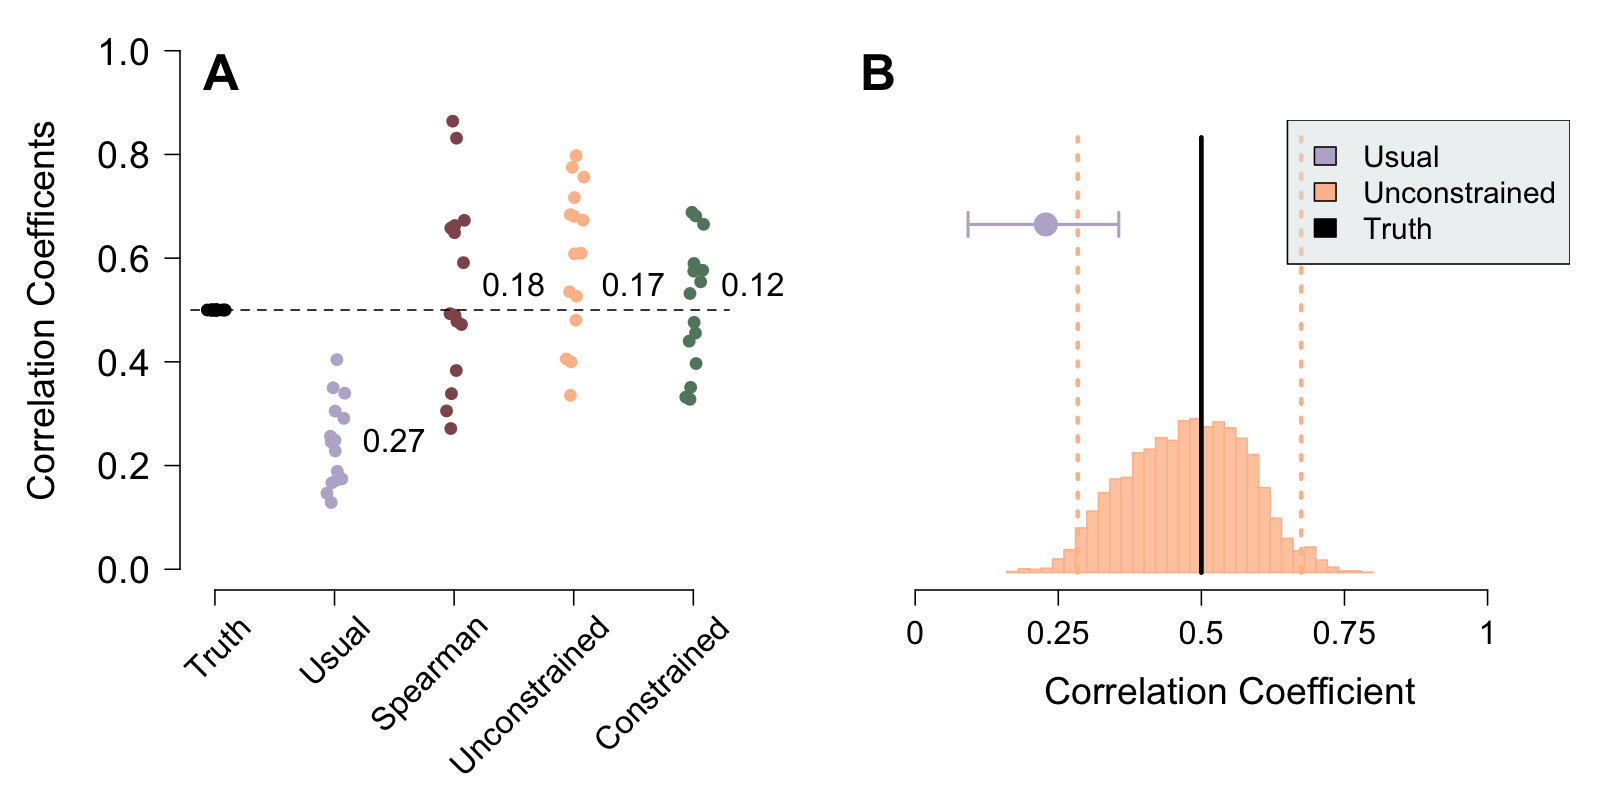
\includegraphics[width=\linewidth, height=1\linewidth, keepaspectratio]{_figs/prob_setupAll.png}
    \caption{A. A single simulation run where all true correlations are .5.  Shown are the usual Pearson sample correlations, the Spearman disattenuated correlations, and estimates from an unconstrained and constrained hierarchical model.  The values next to the spread of points show the RMSEs in estimation.  B. A comparison of uncertainty in correlation estimates.   The point shows the usual estimate along with 95\% confidence intervals.  The distribution shows the posterior of the unconstrained model correlation estimate.  The usual estimate not only is dramatically attenuated, but has narrow CIs that do not cover the true values.  The posterior is centered on the truth, but is wide showing difficulty in localizing correlations without constraint.}  
    \label{fig:prob_setup}
\end{figure}

\begin{figure}[htbp]
    \centering  % Centers the figure
    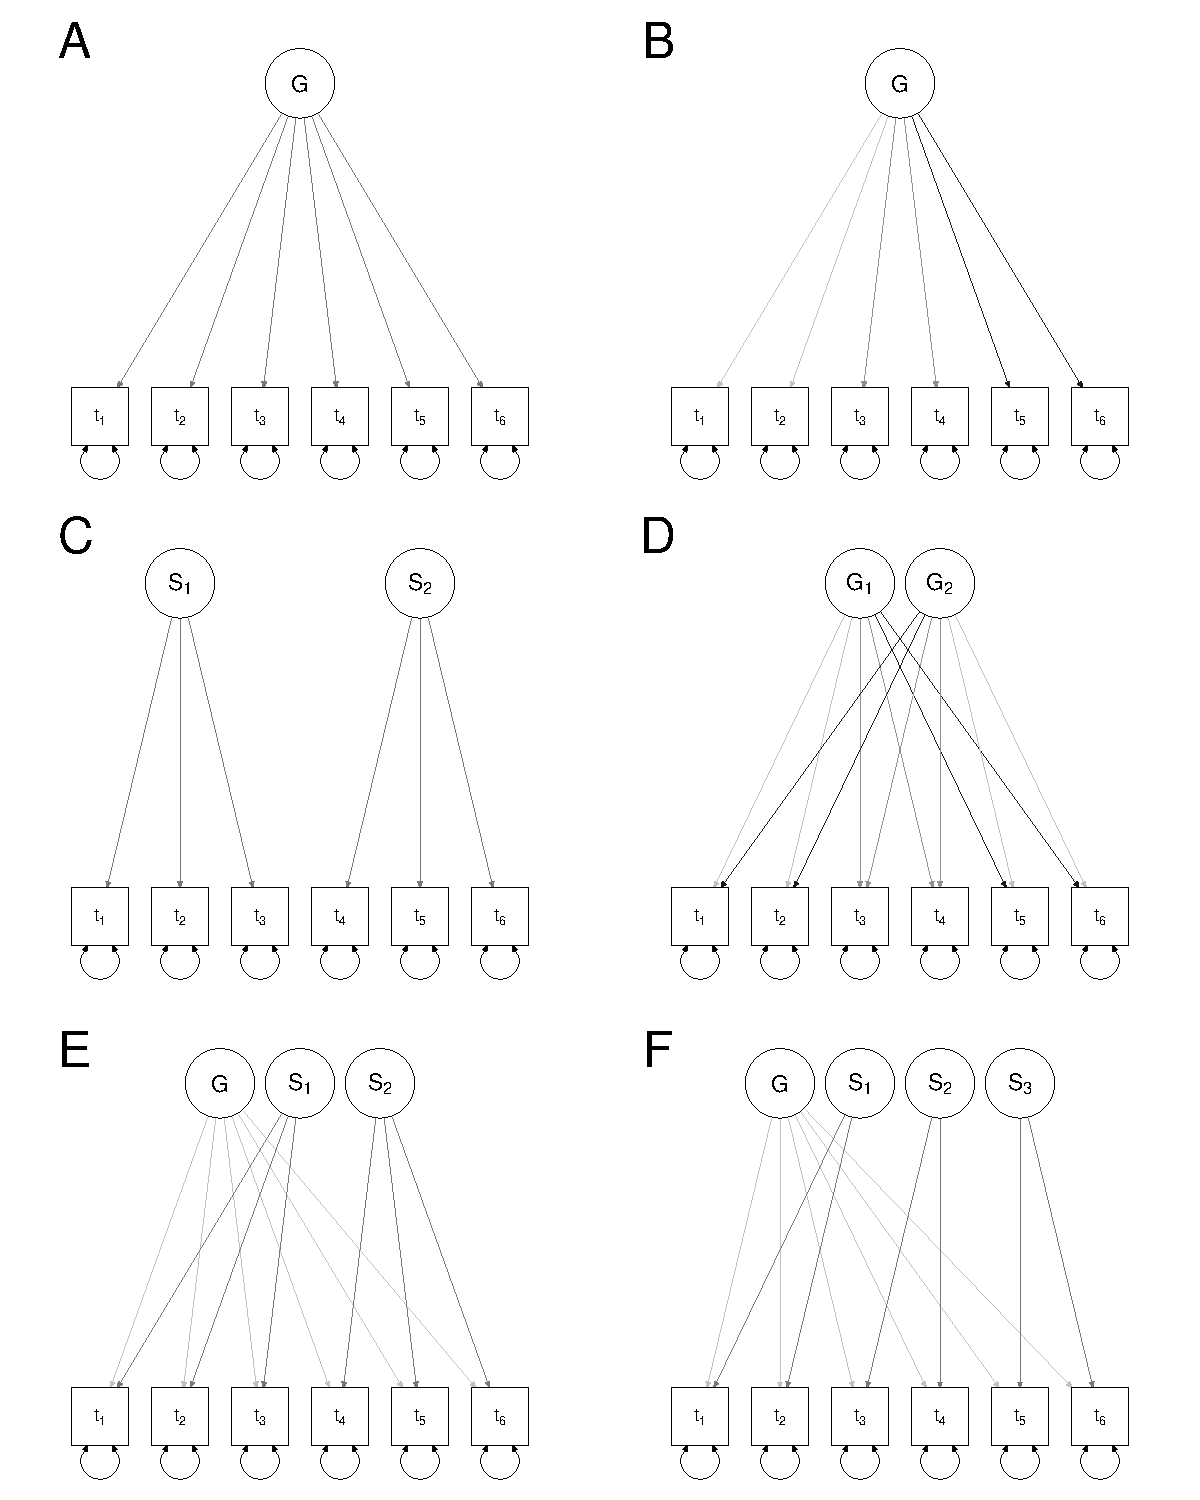
\includegraphics[width=\linewidth, height=1.1\linewidth, keepaspectratio]{_figs/factor_tree.pdf}
    \caption{Latent variable representations of the ground truths used in simulations.  See Figure \ref{fig:true_cors} for the corresponding true correlation matrices.}  % Replace 'TK' with your actual caption.
    \label{fig:fac_st}
\end{figure}



\begin{figure}[htbp]
    \centering  % Centers the figure
    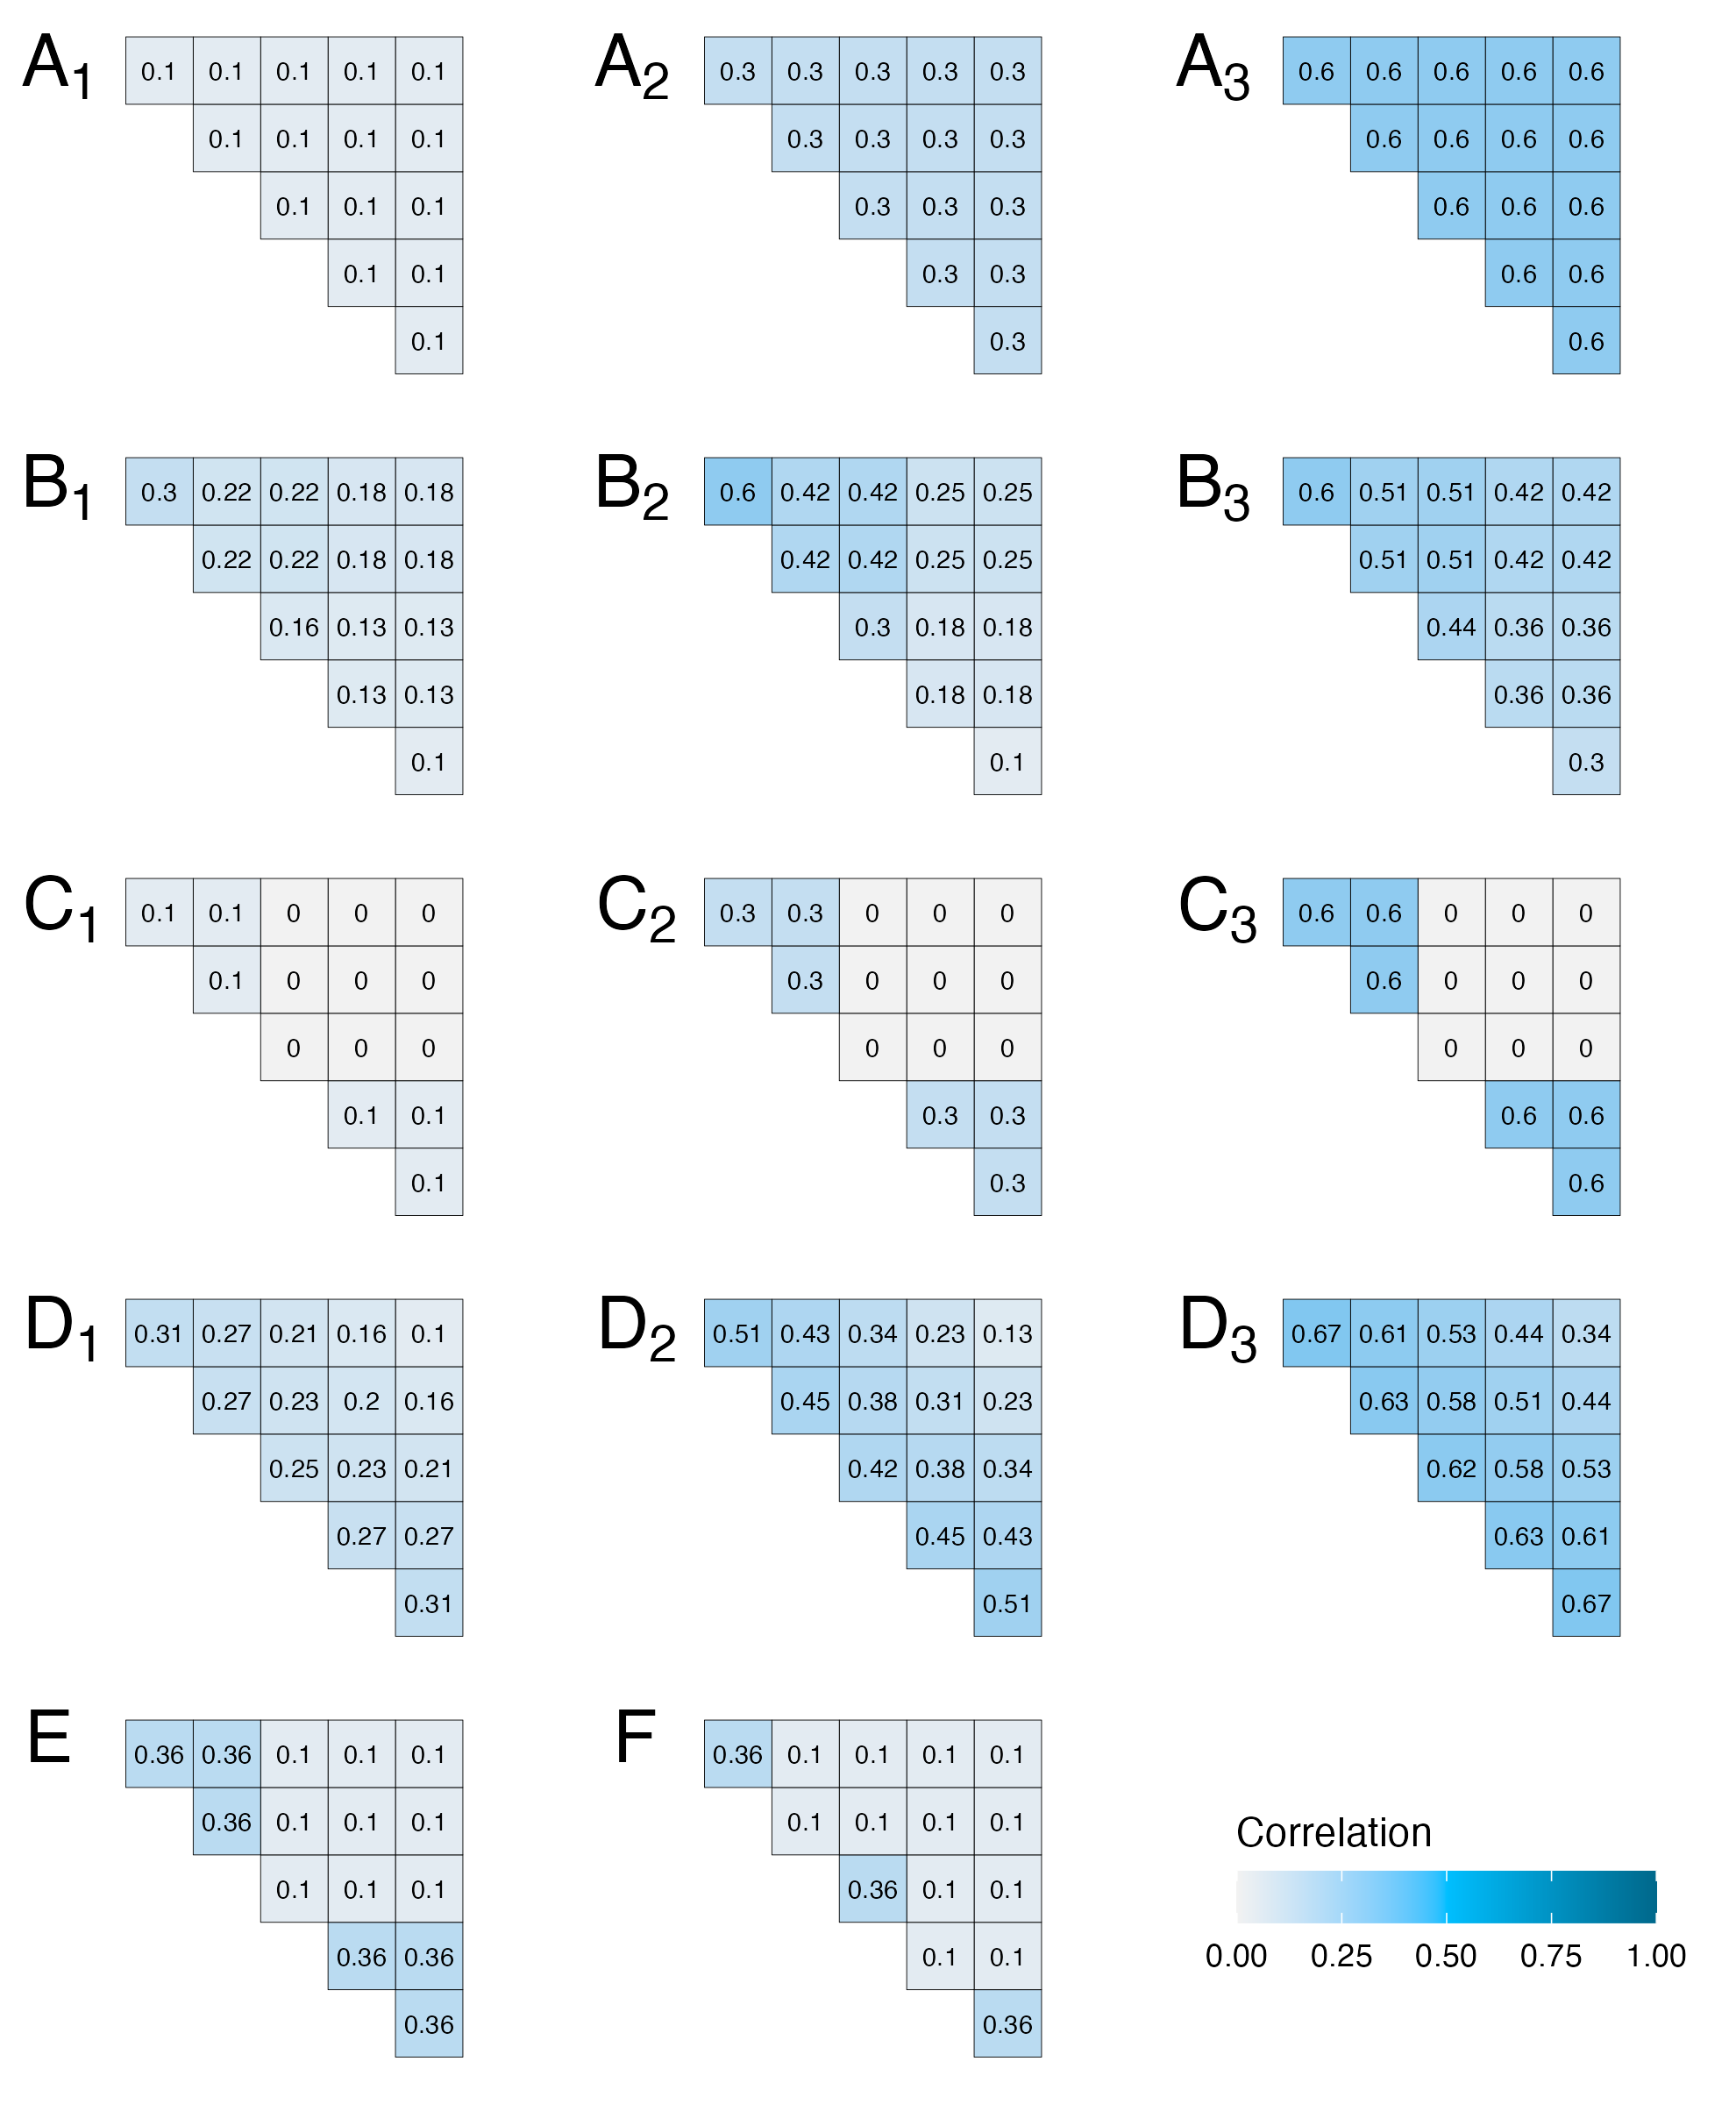
\includegraphics[width=\linewidth, height=1.1\linewidth, keepaspectratio]{_figs/true_cors.png}
    \caption{True correlation matrices across the 14 simulations.  See Figure \ref{fig:fac_st} for the corresponding latent variable representation.} 
    \label{fig:true_cors}
\end{figure}

\begin{figure}[htbp]
    \centering  
    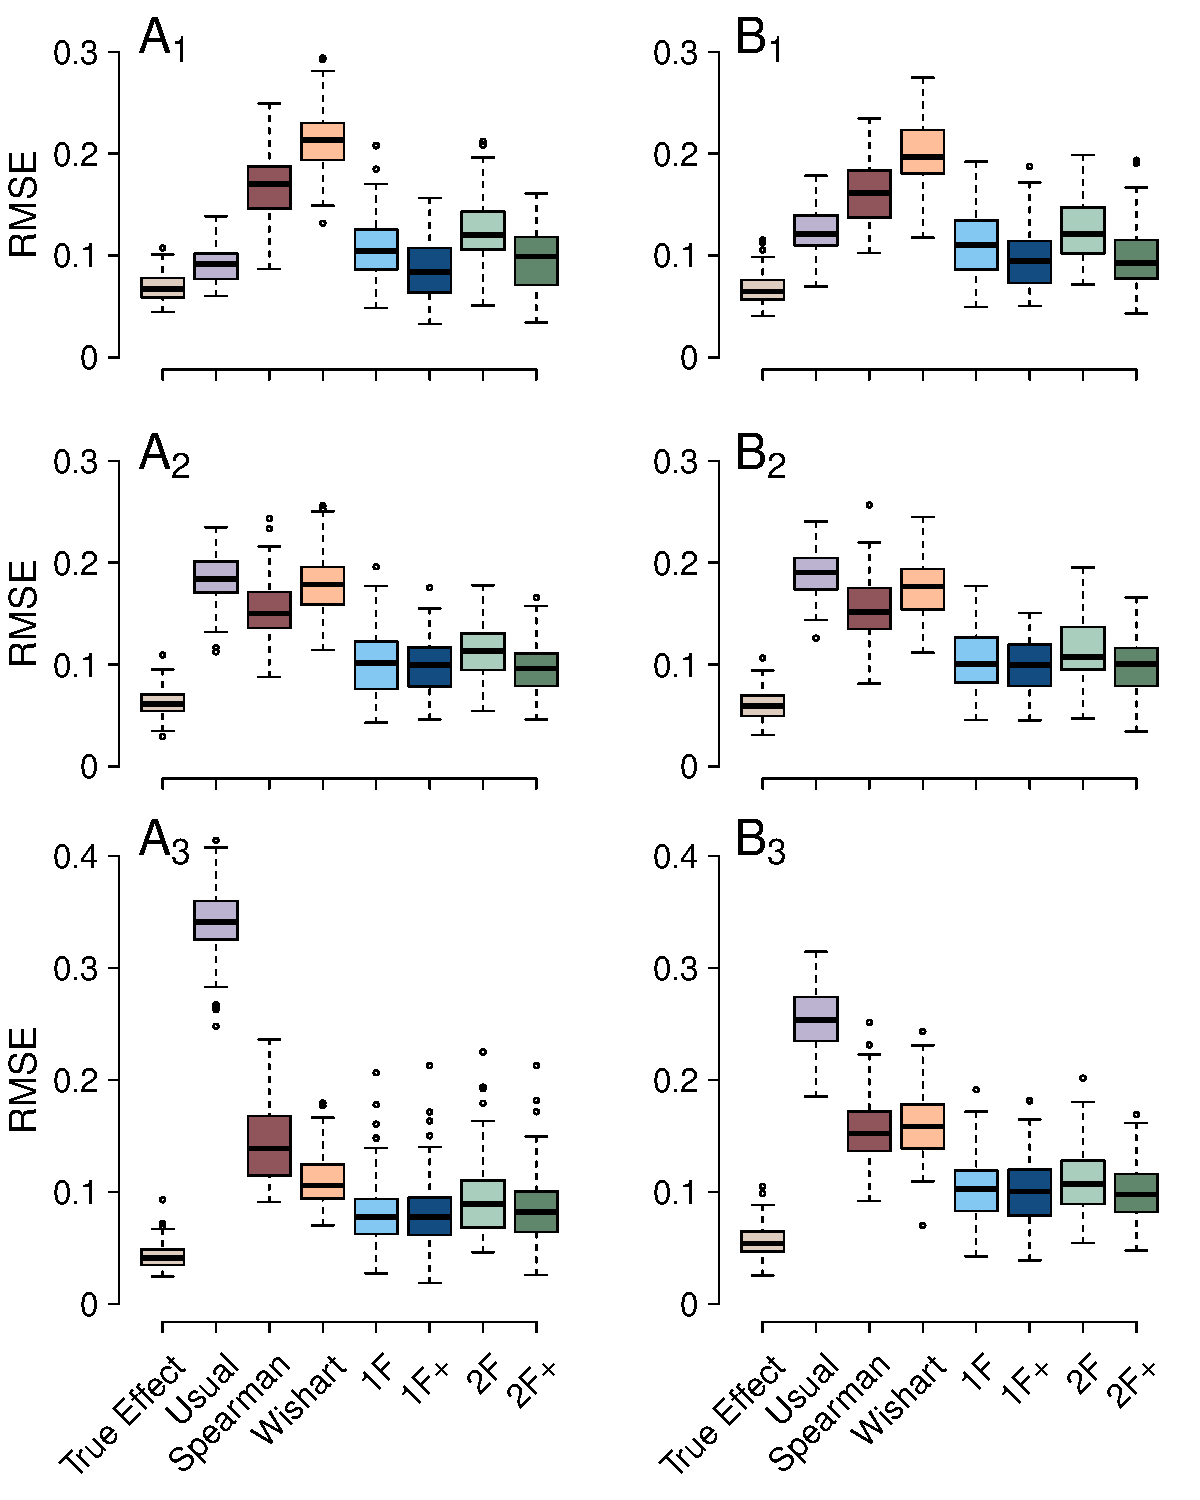
\includegraphics[width=\linewidth, height=1.1\linewidth, keepaspectratio]{_figs/rmse-res1.pdf}
    \caption{Distributions of RMSE across the 108 simulation runs for the six ground truths from the one-factor setup. Panel labels, such as A$_1$, correspond to true correlation matrices in Figure \ref{fig:true_cors}.}  
    \label{fig:rmse-res1}
\end{figure}

\begin{figure}[htbp]
    \centering  
    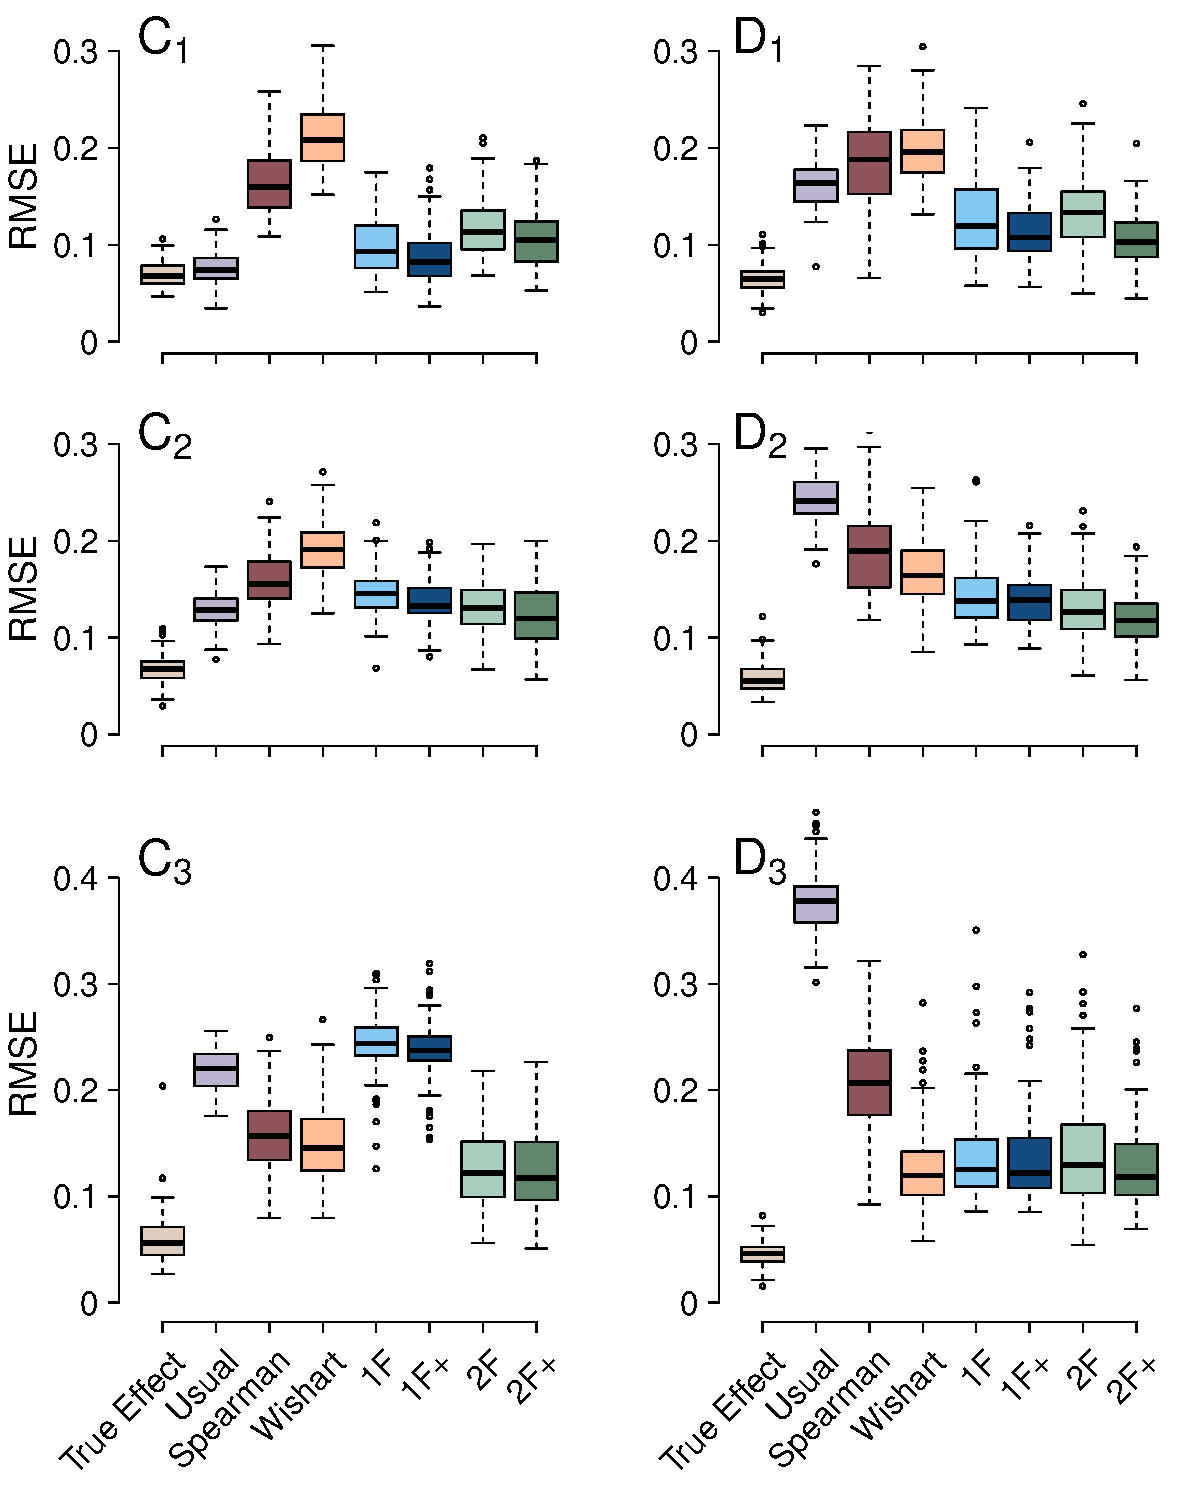
\includegraphics[width=\linewidth, height=1.1\linewidth, keepaspectratio]{_figs/rmse-res2.pdf}
    \caption{Distributions of RMSE across the 108 simulation runs for the six ground truths from the two-factor setup. Panel labels, such as C$_1$, correspond to true correlation matrices in Figure \ref{fig:true_cors}} 
    \label{fig:rmse-res2}
\end{figure}

\begin{figure}[htbp]
    \centering  
    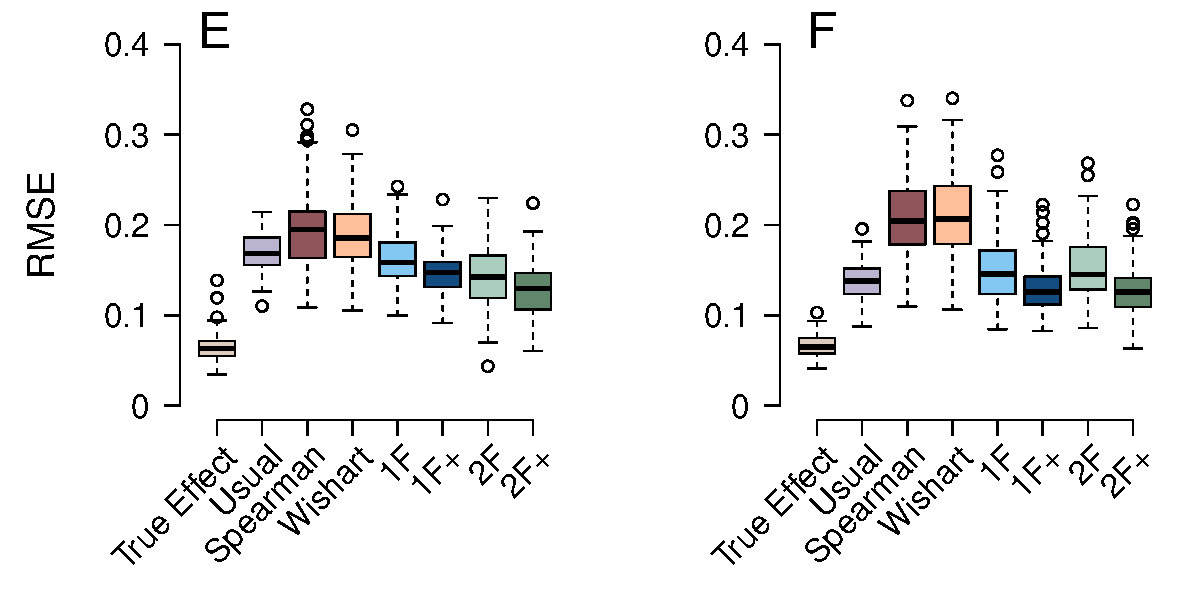
\includegraphics[width=\linewidth, height=1.1\linewidth, keepaspectratio]{_figs/rmse-res3.pdf}
    \caption{Distributions of RMSE across the 108 simulation runs for the two ground truths from the bi-factor setups. Panel labels, such as E, correspond to true correlation matrices in Figure \ref{fig:true_cors}}  
    \label{fig:rmse-res3}
\end{figure}


\begin{figure}[htbp]
    \centering  % Centers the figure
    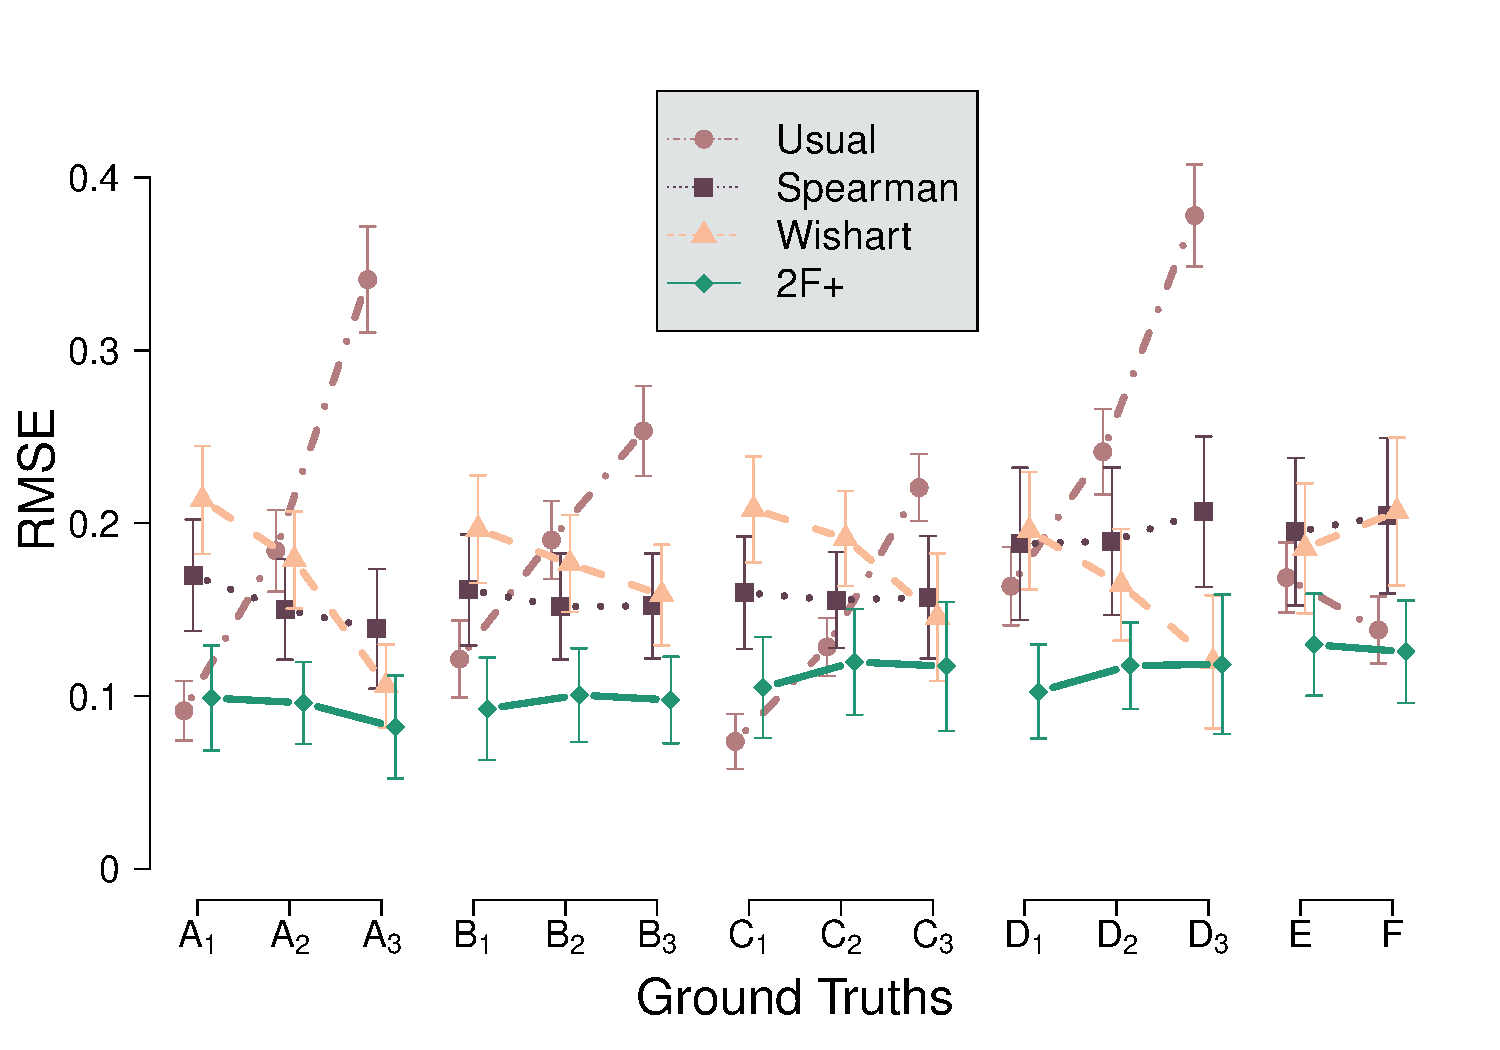
\includegraphics[width=\linewidth, height=1.1\linewidth, keepaspectratio]{_figs/rmse-snap.pdf}
    \caption{Summary of RMSE gain across all ground truths for select estimates. The two-factor positive constraint model does the best, overall, for localizing correlations.} 
    \label{fig:rmse-snap}
\end{figure}

\begin{figure}[htbp]
    \centering  % Centers the figure
    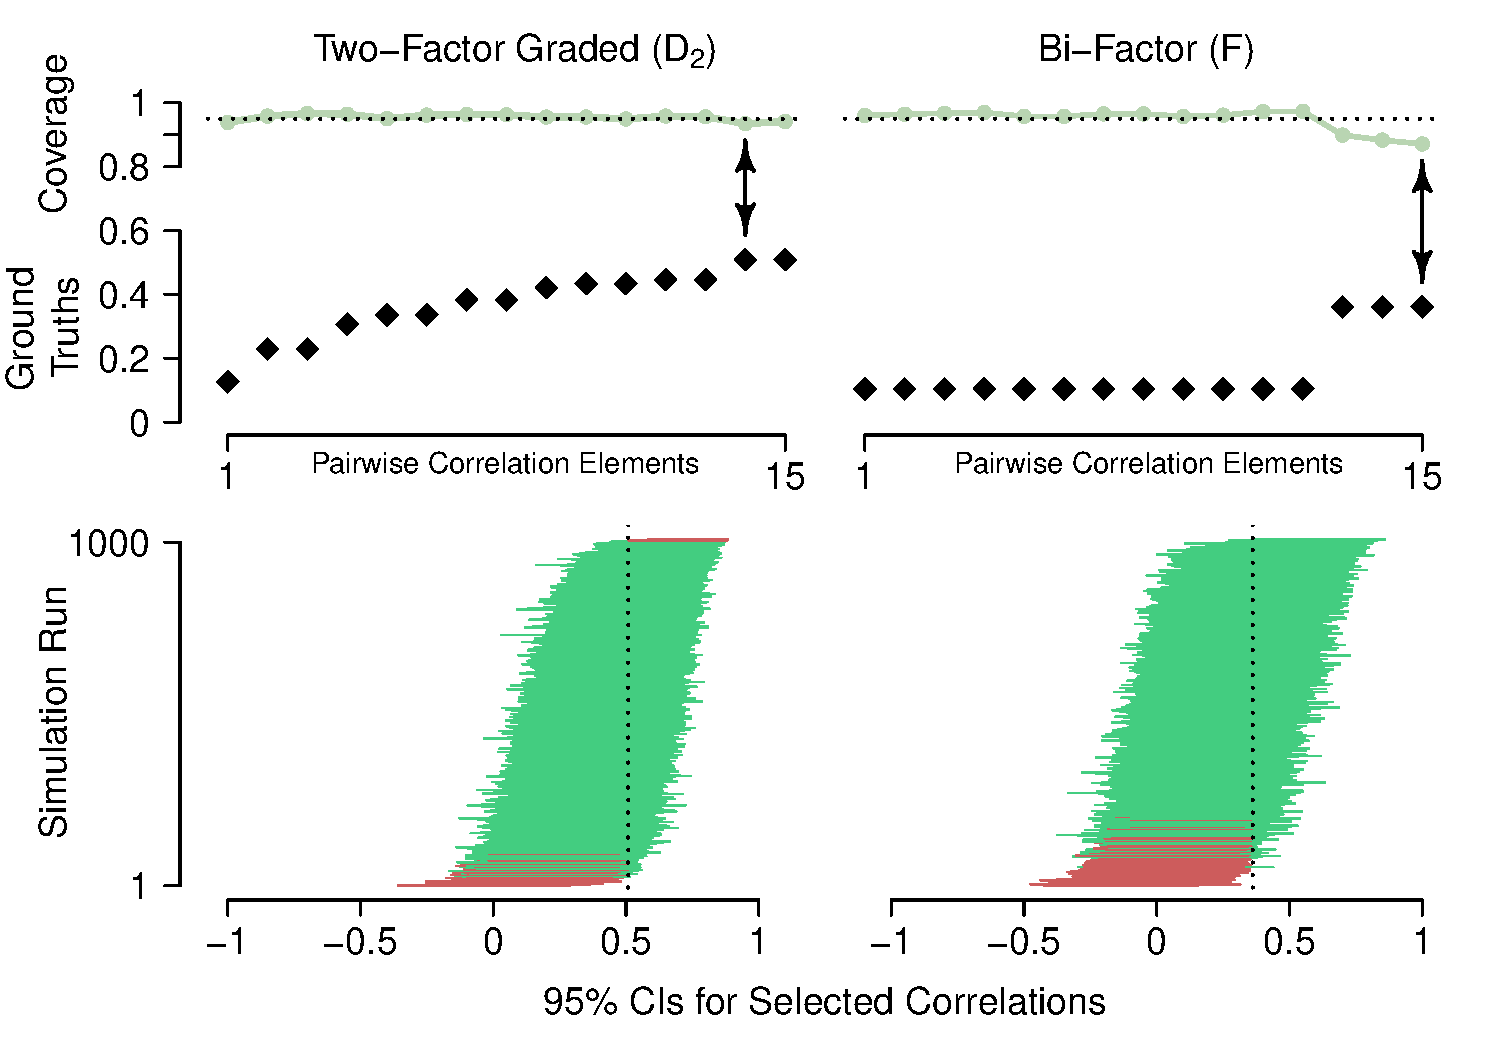
\includegraphics[width=\linewidth, height=1.1\linewidth, keepaspectratio]{_figs/coverage.pdf}
    \caption{Coverage proportions and credible intervals for the two-factor model.  Top: Coverage proportions and true correlation values for the two-factor graded  ground truth (left) and bi-factor ground truth (right).  The arrow indicates true values with the worst coverage.  Bottom: Worst-case distribution of 95\% credible intervals.  There is one CI for each run.  Green and red intervals respectively cover and fail-to-cover true values (black dotted line). These are worst-case distributions because they correspond to the true correlation value with the worst coverage.} 
    \label{fig:coverage}
\end{figure}


\end{document}